
\documentclass[journal]{IEEEtran}

\usepackage[margin=1in]{geometry} 
\usepackage{amsmath,amsthm,amssymb}
\usepackage{enumerate}
\usepackage{graphicx}
\usepackage{caption}
\usepackage{subcaption}
\usepackage{float}
\usepackage{listings}
\usepackage{color}
\usepackage{booktabs}
\usepackage{pgfplots}
\usepackage{tikz}
\usepackage{changes}
%\usepackage[american,siunitx]{circuitikz}
\usepackage[american]{circuitikz}
\usepackage[free-standing-units]{siunitx}
\usepackage{xspace}
\usepackage{mathpazo}
\newcommand\st{\textsuperscript{st}\xspace}



% correct bad hyphenation here
\hyphenation{op-tical net-works semi-conduc-tor}


\begin{document}

\title{MD5 Optimizations: Hardware and Software Implementations}

\author{Danny~Froerer and Taylor~Peterson\\
\textit{Utah State University Department of Electrical and Computer Engineering}}
\maketitle

% As a general rule, do not put math, special symbols or citations
% in the abstract or keywords.
\begin{abstract}
This paper discusses different optimizations of the MD5 hashing algorithm. Basic optimizations include a loop unrolled algorithm and the use of Intel AVX intrinsics. String comparisons, arithmetic changes, and multi-threading were also used. A version of the MD5 was also implemented on a Diligent, Nexys 2 FPGA board demonstrating specific hardware optimizations.  
\end{abstract}

% Note that keywords are not normally used for peerreview papers.
\begin{IEEEkeywords}
MD5, AVX Intrinsics, Hashing 
\end{IEEEkeywords}


\section{Introduction}
\IEEEPARstart{A}{s} there are many implementations of the MD5 hashing algorithm, our goal was to combine different optimization strategies using the C coding language to increase the number of hashes per second. The baseline algorithm used was partially optimized when compared to the most basic version of MD5. The baseline included loop-unrolling and the use of Intel Advanced Vector Extension (AVX) Intrinsics. Other optimizations included string comparisons, arithmetic changes, and multi-threading. These were then appended to the baseline code separately and together to verify that multiple, yet different optimizations could improve the hashes per second rate. A version of MD5 was then written in Verilog and optimized to work specifically on an FPGA. This was done to show that by having a knowledge of the hardware, you can exploit and take advantage of it for a specific purpose.

\section{Software Implementation}
A very basic implementation of the MD5 algorithm was first written in the C programming language. After this basic version was verified to be working, both loop unrolling and AVX intrinsics were introduced into the code.

\subsection{Loop Unrolling and AVX Intrinsics}
Loop unrolling was a very basic and relatively simple optimization. This was done by explicitly stating each instruction inside of a loop thus eliminating extra instructions that control the loop. This increases the size of the program, but it also increases the execution speed of the program.
\newline
A more difficult, but worthwhile optimization was including AVX intrinsics into the code. AVX uses vectors to store information which allows the use of single instruction, multiple data (SIMD) parallel computing. An example of the power of parallel computing can be seen in Figure ~\ref{SIMD}.

\begin{figure}[H]
	\centering
	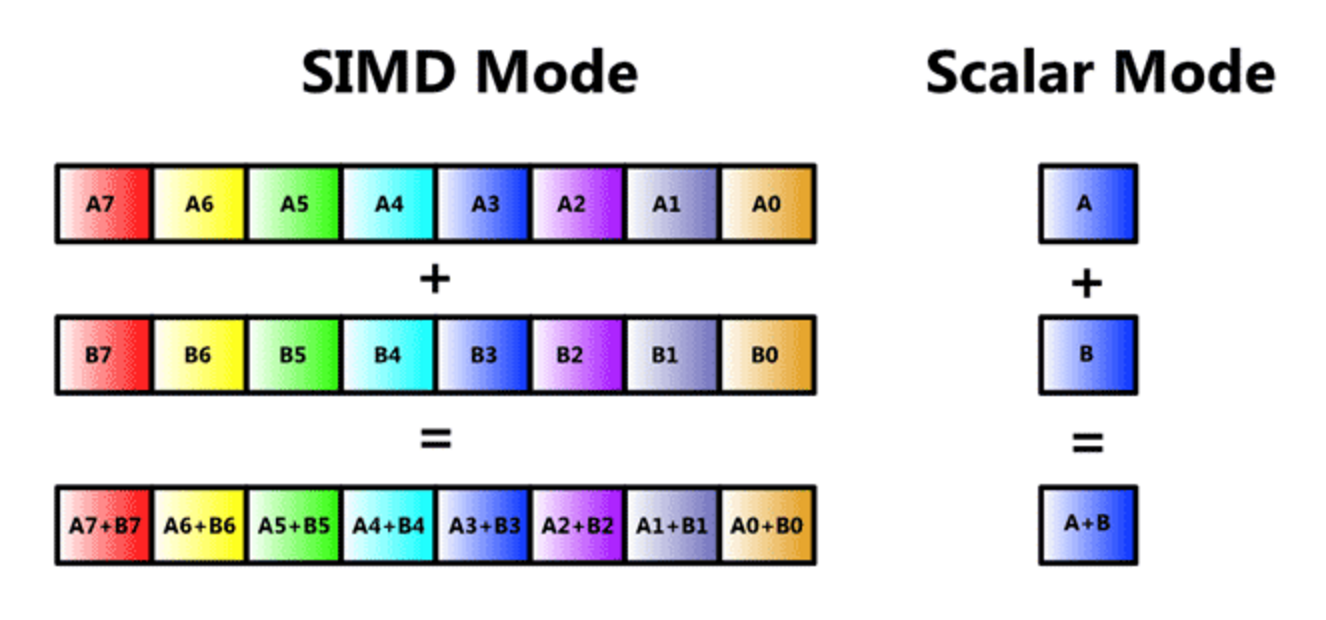
\includegraphics[scale=.30]{SIMD.png}
	\caption{SIMD vs. Scalar Arithmetic \cite{SIMD}}
	\label{SIMD}
\end{figure}

Combining both loop unrolling and the use of AVX intrinsics comprised the baseline version of the code. From that point, other optimizations were implemented used to enhance the code further. 

\subsection{Optimization I}
After reviewing the baseline code, it was decided that when looking for a specific hash, depending on the number of initial candidates, it may not be necessary to compare the whole hash. This is because the hashed output is extremely random, and the probability of just the first half of the hash being equal to another hash is tremendously small. The first optimization implemented was only comparing the first half of the hash to see if there was a match and if not, the program would just continue. There were also a few things implemented to clean up the code further and make it run quicker. Some parenthesis were added to potentially clean up some order of operations and make them quicker as well. After running the code, these optimizations did not improve the speed as much as was hoped for, but they did improve it slightly.

\subsection{Optimization II}
Although Optimization I did not quite as well as was hypothesized, the second optimization added was multi-threading. This worked very well and there was a very significant increase in speed. Multi-threading takes the program and divides it into a specified number of segments and runs different portions of the input at the same time. For example, if the input is 1-100, then with one thread it would run through all 100 inputs while if there were two threads, then one thread would run 1-50 while the other ran 51-100 simultaneously. It is very powerful as seen in the results.

\subsection{Software Results}
The different optimizations were applied to all lowercase passwords of length six, i.e. aaaaaa to zzzzzz. After running the various files separately, the results were summarized in Table ~\ref{hashes}.

\begin{table}[H]
	\centering
	\caption{Performance of Each Optimization in Millions of Hashes/Second}
	\label{hashes}
	\begin{tabular}{@{}lcccc@{}}
		\toprule
		\textbf{Optimization} & \textbf{-O0} & \textbf{-O1} & \textbf{-O2} & \textbf{-O3} \\ \midrule
		Baseline              & 2.97         & -            & -            & -            \\
		Half Comparison       & 3.05         & 6.03         & 7.55         & 7.56         \\
		Threading             & 12.82        & 28.95        & 31.49        & 31.48        \\
		Combined              & 13.33        & 28.93        & 31.35        & 30.04        \\ \bottomrule
	\end{tabular}
\end{table}

\section{Hardware Implementation}
MD5 is fundamentally a simple algorithm. The challenge to password cracking is the time taken to go through the many calculations to get a single hash. A Field Programmable Gate Array (FPGA) is of special interest for this project because of its speed and ease of implementation. FPGAs can be used to create fast reliable program implementations that operate at the hardware level. These devices allow the user to manipulate the configuration of an array of logic blocks to accomplish the desired result. Ultimately, the FPGA is only limited by the size of the logic gate array and other hardware specific features. A design was developed for Xilinx xc3s1200e Spartan 3 as part of the Diligent Nexys 2 development board. The FPGA contains 1200K gates, 19,512 logic cells with a total slice count of 8,672.

\subsection{Architecture}
The FPGA implementation was formed using ISE Project Navigator (P.20131013). The program hashed a single password and checked the solution against the programed target. A successfully matched hash is communicated through an LED output line.  As can be seen in Figure ~\ref{fpga}, the simulation shows a successful relationship between the A, B, C, D outputs of the hash function and the programed target of Aend, Bend, Cend, Dend.

\begin{figure}[H]
	\centering
	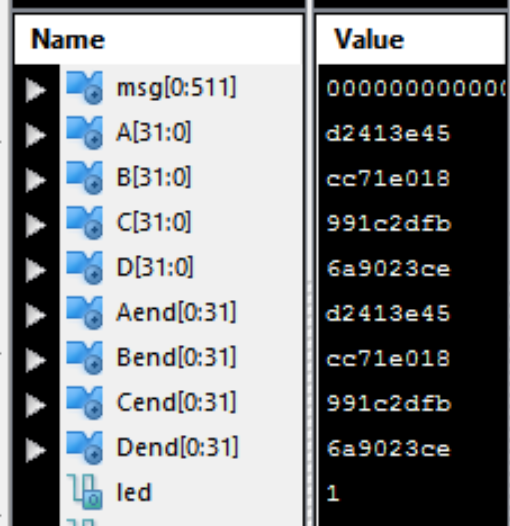
\includegraphics[scale=.30]{fpga.png}
	\caption{Successful FPGA Implementation}
	\label{fpga}
\end{figure}

The program was broken into basic modules. The most basic modules included individual functions for the four rounds of the hash function involving the F, G, H, and I equations. Coding was simplified by using implicit declarations such as $result = (a + F(b,c,d) + m + t)$; and functions such as $F = (x\&y)|(\neg x\&z)$;. This method of Verilog programming minimized the amount of explicit modules needed such as barrel shifters and 32 bit adders.

The code was designed for optimum throughput by loop unrolling the function rounds. The individual rounds were declared and synthesized for the FPGA to minimize the need for logical overhead calculations. These rounds were then directly wired into the next round in a shifted order to also minimize the extra overhead of the shifting steps. This method requires additional gates in exchange for increased speed.

The speed for gates exchange is a method that holds true and is only limited by the number a gates. Theoretically, this method of implementing a hashing algorithm could be expanded on a larger FPGA or even onto many FPGAs for a throughput much greater than a CPU. Of course, this method would also include additional overhead and cost. 

\section{Conclusion}
It was shown that by using different optimizations in the software, much greater speeds can be reached. The results show that combining both of the optimizations was slightly slower for the complier optimizations, but just running it straight, it is the most optimized. Also, by understanding the hardware, greater speeds can be achieved as well.

\ifCLASSOPTIONcaptionsoff
  \newpage
\fi

\begin{thebibliography}{1}

\bibitem{SIMD}
C.~Lomont. (2011, June 21). \emph{Introduction to Intel Advanced Vector Extensions}[Online]. Available: https://software.intel.com/en-us/articles/introduction-to-intel-advanced-vector-extensions 

\end{thebibliography}

\end{document}


